\section{The model}
\label{sec:the-model}
In this section we will go through the model presented in \cite{self-org} in 
detail. As mentioned in the introduction, social force models are agent-based, 
that is they describe the system by looking at the behaviour of each agent or, 
in our case, pedestrian in the system.


In this model the behaviour each pedestrian is defined by a series of social 
forces. We will describe three main forces, that each represent a tendency of 
the pedestrians. These forces are \emph{the desired movement force},  
\emph{the interaction force} between pedestrians and \emph{the repulsive 
force}  from the walls. The model also contains an attractive force, allowing 
e.g. a group of pedestrians to stick together when moving around, and a 
fluctuation term, adding a stochastic quality to the model. Both these forces, 
however, are only mentioned in the article, and are not really used. We have 
written the authors of the article asking about this, and they have replied 
that these parts of the model have not been used in practice, but that they 
might be useful to include at a later point in time.  Because of this, we will 
exclude these parts from the explanation of the model.

In the following, we will go through the three main forces, explaining how 
they are calculated. Since the notation used in the article is ambiguous and 
confusing, we introduce our own notation in an attempt to make it clearer. We 
will not refer to the original notation, but only use our own.


In the model, a pedestrian is represented by a circle with a centre, a radius 
and a current velocity. Walls are represented as line segments. The desired 
direction is represented by assigning to each pedestrian a target to move 
towards. Various other parameters are assigned to each pedestrian; these will 
be explained when relevant throughout the description. The notation for 
pedestrians and the main forces acting on a pedestrian are illustrated in  
figure~\ref{pedestrian-notation}.  

\begin{figure}[ht]
    \centering
    \subfloat[Notation of pedestrian properties.]{
        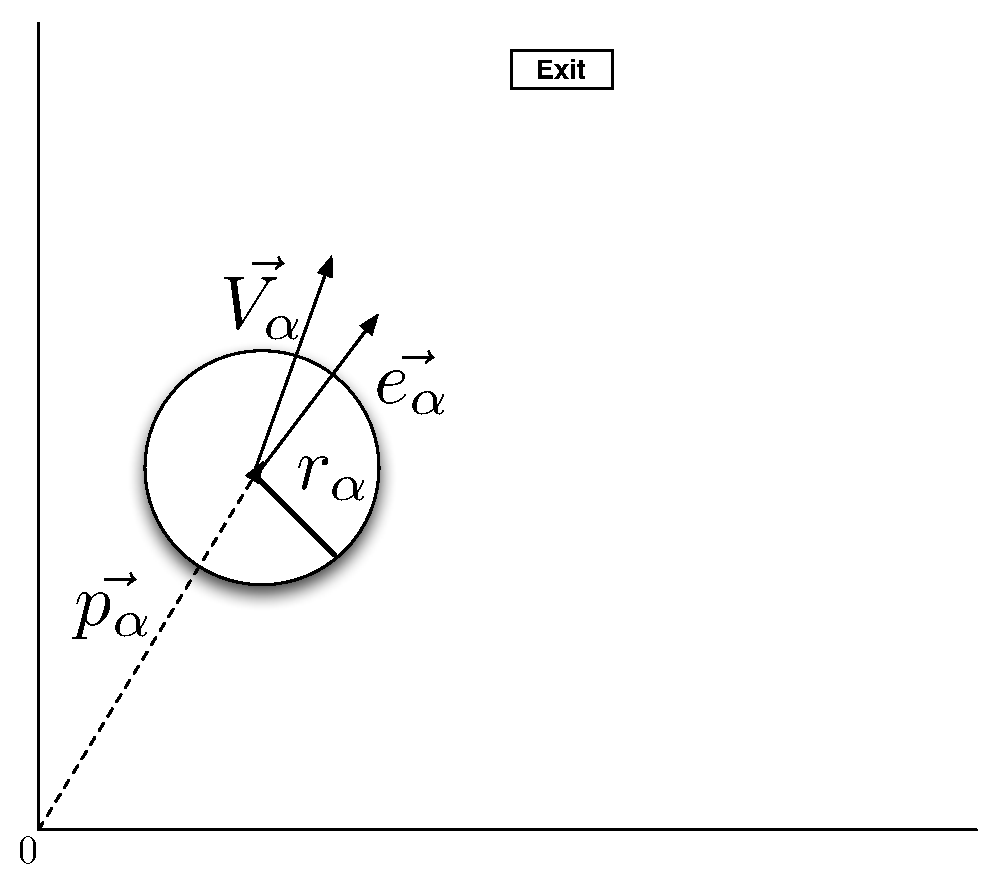
\includegraphics[width=0.45\textwidth]{Figures/NotationOfPedestrian.pdf}
        \label{subfig:notation}
    }
    \subfloat[Main forces acting on a pedestrian.]{
        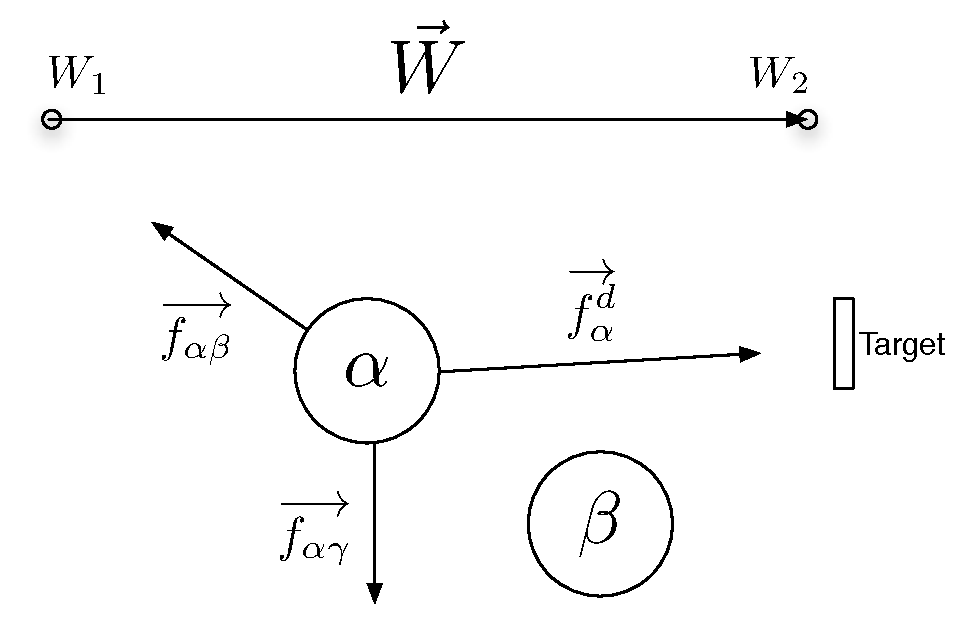
\includegraphics[width=0.45\textwidth]{Figures/ForceModel.pdf}
        \label{subfig:forces}
    }
    \caption[Notation for pedestrians]{Notation for a pedestrian.  
    \subref{subfig:notation} The notation for pedestrian properties. Position 
    vector ($ \overrightarrow{p_{\alpha}} $), velocity vector ($ 
    \overrightarrow{V_{\alpha}} $), vector pointing towards 
    the target ($\overrightarrow{e_{\alpha}}$)  and radius ($ R_{\alpha} $).
    %
    \subref{subfig:forces} Main forces acting on a pedestrian $\alpha$. 
    Repulsive force from pedestrian $\beta$ 
    ($\overrightarrow{f_{\alpha\beta}}$), repulsive force from wall $\gamma$ 
    ($\overrightarrow{f_{\alpha \gamma}}$) and desired force towards target 
    ($\overrightarrow{f^{d}_{\alpha}}$).}

    \label{pedestrian-notation}
\end{figure}

The resulting force for pedestrian $\alpha$, $\overrightarrow{f_{\alpha}}$ is 
the sum of the three main forces.

\begin{equation}\label{model}
    \overrightarrow{f_{\alpha}} = \overrightarrow{f^{d}_{\alpha}} +
    \sum_{\gamma} \overrightarrow{f_{\alpha \gamma}} +
    \sum_{\beta \neq \alpha} \overrightarrow{f_{\alpha \beta}}
\end{equation}

Here $\overrightarrow{f_{\alpha}^{d}}$ is the desired force, 
$\overrightarrow{f_{\alpha \gamma}}$ is the repulsive force from wall $\gamma$ 
and $\overrightarrow{f_{\alpha \beta}}$ is the repulsive force from pedestrian 
$\beta$. The main forces are summarised in table~\ref{tbl:main-forces} and 
will be described in detail in the following sections.

\begin{table}[h]
    \centering
    \begin{tabular}{l l}
        \toprule
        $\overrightarrow{f_{\alpha}^{0}}$ & the desired force\\
        $\overrightarrow{f_{\alpha B}}$ & the repulsive force from walls\\
        $\overrightarrow{f_{\alpha \beta}}$ & the repulsion from other pedestrians\\
        \bottomrule
    \end{tabular}
    \caption{Summary of main forces.}
    \label{tbl:main-forces}
\end{table}

\subsection{The desired force}
\label{sec:desired-force}
The first term on the right hand side of equation \eqref{model} describes the 
\emph{willingness} of pedestrian $\alpha$'s to reach the exit. It is a velocity 
dependent force and is given by:

\begin{equation}\label{relaxtime}
	\overrightarrow{f^{0}_{\alpha}}\left( \overrightarrow{V_{\alpha}} \right) =
    \frac{1}{\tau}
    \left( V_{\alpha}^{0} \overrightarrow{e_{\alpha}} - \overrightarrow{V_{\alpha}} \right)
\end{equation}

Where $V_{\alpha}^{0}$ is the desired speed, $ \overrightarrow{e_{\alpha}} $ is the unit 
vector pointing in the desired direction of the pedestrian which in most cases will 
be the exit, but it can in principle be anywhere.  $\overrightarrow{V_{\alpha}}$ is the 
actual velocity of the pedestrian, and $\tau$ is the \emph{relaxation time}.

The relaxtion time determines how reactive a pedestrian is. In principle the 
relaxation time can vary for each pedestrian but from the article \cite{self-org} 
we get that $ \tau_{\alpha}\approx 1s $, which means that it takes the pedestrian 
one second to change its velocity. $V_{\alpha}^{0} \overrightarrow{e_{\alpha}}$ is the desired 
velocity of the pedestrian. The desired speed can vary over time and is given by:

\begin{equation}\label{v0eta}
    V_{\alpha}^{0}\left( t \right) = \left[ 1 - \eta_{\alpha} \left( t \right) \right] 
    V_{\alpha}^{0} \left( 0 \right) +
    \eta_{\alpha} \left( t \right)V_{\alpha}^{\text{max}}
\end{equation}
%TODO: write that V_a^0(0) < V_a^0(t) < V_a^max
where $V_{\alpha}^{0} \left( 0 \right)$ is the desired speed at $ t=0 $, and 
$V_{\alpha}^{\text{max}}$ is the maximum desired speed of pedestrian $\alpha$. The 
maximum desired speed is the speed that pedestrian $\alpha$ will try to get if it 
is allowed by the environment and other pedestrians. It is not a physical limit to 
how fast the pedestrian can move but rather a parameter that determines the speed 
that the pedestrian is comfortable walking with. 

$\eta_{\alpha} \left( t \right)$ is called the impatience or nervousness of 
the pedestrian and is given by:

\begin{equation}\label{eta}
	\eta_{\alpha} \left( t \right) =
    1 - \frac{\overline{V}_{\alpha} \left( t \right)}
             {V_{\alpha}^{0} \left( 0 \right)}
\end{equation}

where $\overline{V}_{\alpha}\left( t \right)$ is the average speed in the 
desired direction.Excately how one measures the average speed in the desired 
direction is not properly explained in the article. We define it to be the 
projection of the position vector $ \overrightarrow{p_{\alpha}} $ onto the desired direction 
of motion $e_{\alpha}$ devided by the time that the simulation has run. A 
illustration of this can be seen i figure \ref{impatience}. The mathematical 
expression becomes:

\begin{figure}[ht]
    \centering
    {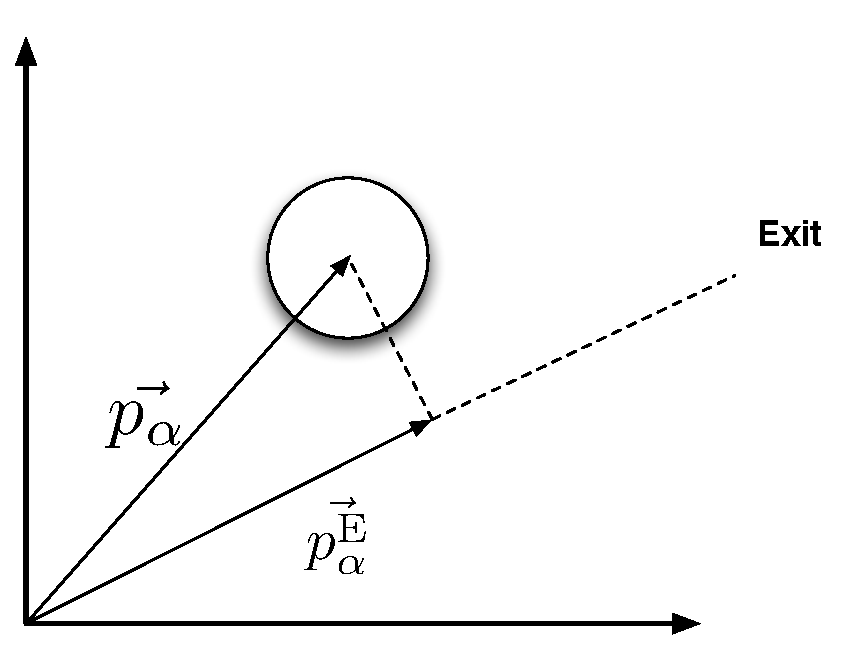
\includegraphics[scale=0.35]{Figures/NotationOfPedestrian2.pdf}} 
    \caption{Illustration of the vector $ \vec{p_{\alpha}^{E}}$, which is the projection of $ \vec{p_{\alpha}} $ onto the desired direction of motion.}
    \label{impatience}
\end{figure}

\begin{equation}\label{averagespeed}
   \overline{V}_{\alpha} \left( t \right) =
   \frac{1}{t} \overrightarrow{p_{\alpha}}\cdot \overrightarrow{e_{\alpha}} 
\end{equation}

$\overline{V}_{\alpha}$ is undefined at $t=0$ beacause that would mean 
that you should divide by zero, which is undefined. This in turn means 
that $\eta_{\alpha}(0)$ is undefined. We therefore define 
$V_{\alpha}^{0}(t)$ for $t=0$ and $t>0$ to be the following:

\begin{equation}\label{eqn:cond-define}
  V_{\alpha}^{0} (t) = \left\{ 
  \begin{array}{l l}
    V_\alpha^0(0) & \text{if $t=0$}\\
    \left[ 1 - \eta_{\alpha} \left( t \right) \right] 
    V_{\alpha}^{0} \left( 0 \right) +
    \eta_{\alpha} \left( t \right)V_{\alpha}^{\text{max}} & \text{if 
    $t > 0$}\\
  \end{array} \right.
\end{equation}
% TODO: This definition is a tautology. We need a different notation for 
% initial desired velocity.

If we look at the expression for $V_{\alpha}^{0}$ for $t>0$ we can 
start to analyse how this affects the behaviour of the pedestrian. There 
are three cases that is of interests, namely $0 < \eta_{\alpha} < 1$, 
$\eta_{\alpha} < 0$ and $1 < \eta_{\alpha} $.

In the case where $0 \leq \eta_{\alpha} \leq 1$ the expression for 
$V_{\alpha}^{0} \left( t \right)$ makes a lot of sense. Here we can see why this term 
is called the impatience of the pedestrian. If the fraction  between the average 
speed in the desired direction and the initial desired speed is low then 
$\eta_{\alpha} \approx 1$. 
When the impatience term is close to one $V_{\alpha}^{0} \left( t \right)$ is 
dominated by $V_{\alpha}^{\text{max}}$. That is, if the pedestrian have not moved 
very far in the desired direction compared to the initial speed the impatience 
of the pedestrian will cause the pedestrian's future velocity to be dominated by the 
maximum desired velocity of the pedestrian. 
If the pedestrian has been moving in the desired direction with his initial speed 
the entire time then $\eta_{\alpha} = 0$  and $V_{\alpha}^{0} \left( t 
\right)$ will continue to be $V_{\alpha}^{0} \left( 0 \right)$. 

However in the case where $\eta_{\alpha} < 0$, that is the pedestrian has moved 
further in the desired direction than he would have had he been walking with his 
initial speed. This can happen in situations where then pedestrian is being pushed 
forward forward by the crowd.

In the case where $1 < \eta_{\alpha}$ that is the pedestrian has moved further 
in the opposite direction than the desired one. Then can happen if the pedestrian 
starts out by being very close to another pedestrian. However this is not something 
that we think will happen very often. In any circumstances it will only have an 
effect very early in the simulation. 

We see that desired force is mainly controlled by the two parameters $V_{\alpha}^{0} (0)$, 
$V_{\alpha}^{\text{max}}$ and $\overline{V_{\alpha}}$.

This concludes the explanation of the first of the four physical forces. The next 
force in the equation is the repulsive force from the walls.

\begin{center}
\begin{tabular}{lll}
\hline
$\overrightarrow{V_{\alpha}}$ & The actual velocity of pedestrian alpha &\\
\hline
$V_{\alpha}^{0}(t)$ & The desired speed of pedestrian alpha &\\
\hline
$V_{\alpha}^{0}(0)$ & The initial desired speed of pedestrian alpha &\\
\hline
$\overline{V_{\alpha}(t)}$ & The average speed of pedestrian alpha &\\
\hline
$\overrightarrow{p_{\alpha}}$ & The position vector of pedestrian alpha\\
\hline
$e_{\alpha}$& The desired direction of pedestrian alpha\\
\hline
$\tau$& The relaxation time &\\
\hline
\end{tabular}
\end{center}

\subsection{Repulsion from other pedestrians}
The third term on the right hand side of equation \eqref{model} is a summation of all the 
force between pedestrian $\alpha$ and pedestrian $\beta$. The equation we use is taken from a newer article \cite{ABconstant}. We did this because the original article contains two constants that is not given in the articel and in a mail we were adviced, by the authors, to use the values and equation from the new article. 

The function for the repulsion between pedestrians depends on the position vector and the velocity of 
both pedestrians, and it is given by:

\begin{equation}
        \overrightarrow{f_{\alpha \beta }}\left( t \right) = w\left(\phi_{\alpha \beta}\right)\overrightarrow{g}\left(d_{\alpha \beta}(t)\right)
    \label{eq:pedestrianinteraction}
\end{equation}

The two functions that gives the repulsion between the pedestrians is respectively the angel dependece, $ w\left(\phi_{\alpha \beta}\right)$, and the pure force without any angle dependence, $\overrightarrow{g}\left(d_{\alpha \beta}(t)\right)$.

$ w\left(\phi_{\alpha \beta}\right)$ is given as: 

\begin{equation}
    w\left(\phi_{\alpha \beta}\right)=
    \left(
        \lambda_{\alpha} + \left(
            1 - \lambda_{\alpha}
        \right)
		\frac{1+\cos{\phi}}{2}
    \right) 
    \label{angleAB}
\end{equation}

the angle $\phi_{\alpha \beta}$ is the angle between the 
vector pointing from pedestrian $\beta$ to $\alpha$ and the direction in which 
pedestrian $\alpha$ is moving. Cosine to the angle is 

\begin{equation}
\cos \left( \phi \left( t \right) \right)
		= 
	- \overrightarrow{\eta_{\alpha \beta}}
		\left( t \right) 
	\cdot 
\overrightarrow{e_{\alpha}}\left( t \right)
\end{equation}

$\lambda_{\alpha}$ is governing a persons tendency to focus on things happening in front of him 
rather than behind him. It will have a value  $0\leq \lambda_{\alpha}\leq 1$

A value of $\lambda_{\alpha}=1$ means that the force won't depend on the angle. Thus $\alpha$ will react the same to $\beta$ no matter if $\beta$ is in the front or comes from the side or back. A value of $0$ will on the other hand give the maximum angle dependence. We find that $0\leq w\left(\phi_{\alpha \beta}\right)\leq1$ when $-1 \leq \cos \left( \phi \right) \left( t \right) \leq 1$. From this we see that $\alpha$ wont be affected at all if $\beta$ is coming from behind and the force will be maximum when $\beta$ comes directly in the front. It should be noted that in general one will find that the maximum of $w\left(\phi_{\alpha \beta}\right)$ always will be $1$ and the minimum will be equal to $\lambda_{\alpha}$. In very high density calculations $\lambda_{\alpha}$ is often put to $1$, removing $w(\phi_{\alpha \beta})$ and speeding up the simulations.   

% we should make a drawing of this.

The force, without the effect of $w\left(\phi_{\alpha \beta}\right)$, is given as the second term, in the right hand side of equation \ref{eq:pedestrianinteraction}. The function is:  

\begin{equation}
	\overrightarrow{g} 
	\left(
	d_{\alpha \beta}
	\right)
	=
	 A_{\alpha} e^{ \left(\frac{ R_{\alpha \beta} - d_{\alpha \beta}}{B_{\alpha}}\right)}
	\overrightarrow{n}_{\alpha \beta}
	        \label{re}	
\end{equation}

Here $A_{\alpha}$ and $B_{\alpha}$ are constants that can differ for each pedestrian. 
$R_{\alpha \beta}$ is the sum of the radii of $\alpha$ and $\beta$ that is 
$R_{\alpha \beta} = R_{\alpha} + R_{\beta}$. $d_{\alpha \beta}$ is the 
distance from the center of pedestrian $\alpha$ and the center of 
pedestrian $\beta$ and is therefore given by $d_{\alpha \beta} = 
\|\overrightarrow{p_{\alpha}}\left( t \right) - \overrightarrow{p_{\beta}}\left( t \right) \|$.
$\eta_{\alpha \beta}$ is the unit vector pointing from $\alpha$ to $\beta$ 
and it is given by:

\begin{equation}
    \eta_{\alpha \beta} =
        \frac{\overrightarrow{p_{\alpha}}(t) - \overrightarrow{p_{\beta}}(t)}
             {\|\overrightarrow{p_{\alpha}}(t) - \overrightarrow{p_{\beta}}(t) \|}
\end{equation}

\begin{figure}[ht]
    \centering
    {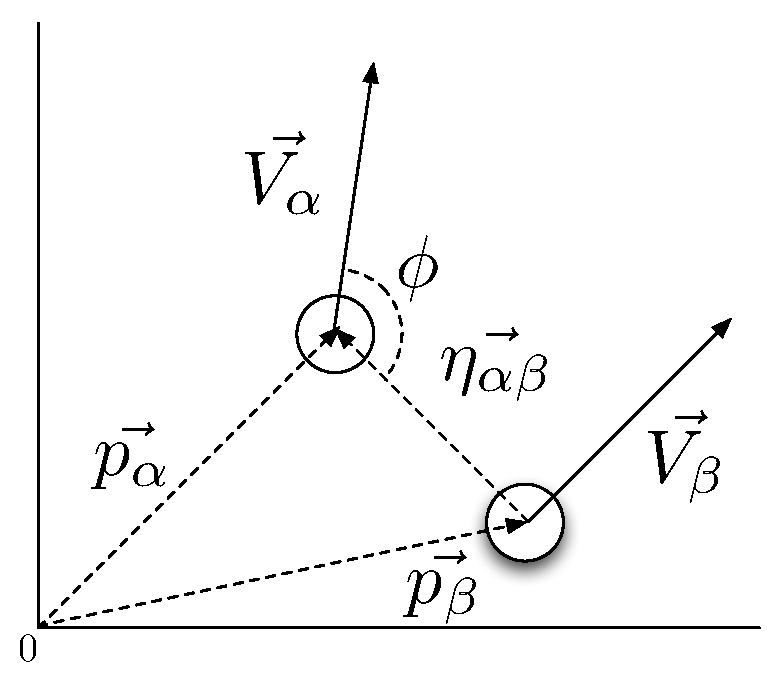
\includegraphics[scale=0.35]{Figures/NotationOfInteraction.pdf}} 
    \caption[Notation of the interaction between two pedestrians]{Illustration of the notation for the interaction between pedestrians.
	     An addition and difference to \ref{NotationOfWall} is that the wall has been replaced by pedestrian $\beta$.
	     $\eta_{\alpha \beta}$ is the vector pointing from $\alpha$ to $\beta$, and $\phi$ is the angle between $\alpha$'s 
	     velocity vector and the vector to $\beta$.}
    \label{fig:NotationOfInteraction}
\end{figure}


%Equation \ref{pedestrianinteraction} is given by two terms. 
%The first term determines how much the the angle between the pedestrians is and how much this angle should affect the force. 
%The constant $\lambda$ is the one controling the importance of the angle.
%The second term reflects the pedestrians tendency to stay at a certain distance 
%from other pedestrians. The constants $A_{\alpha}$, $B_{\alpha}$ is the strength 
%and range of the interaction respectively and controls how big the force will be at a certain distance.  

Taking the norms of both sides of Equation (\ref{re}), we can draw the relation between the value of $\overrightarrow{f_{\alpha\beta}}(t)$ and $ d_{\alpha\beta} $, as shown in Figure 
(\ref{fig:physicalinteraction2}).\\

\begin{figure}[hb]
    \centering
    {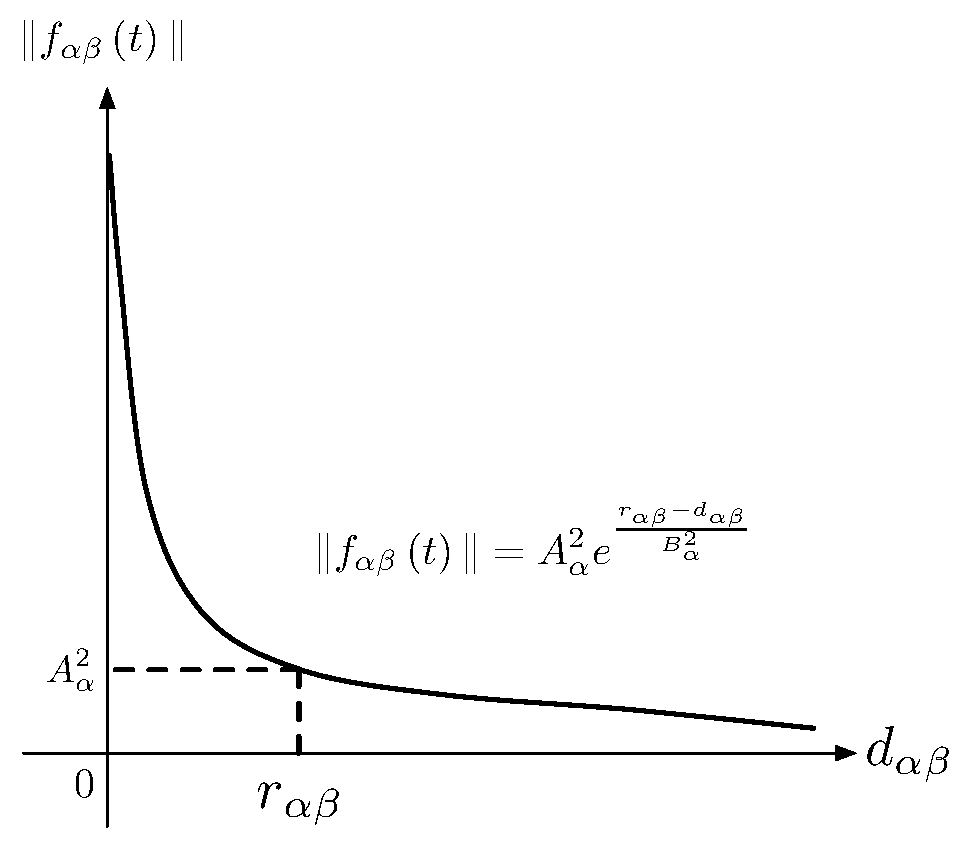
\includegraphics[scale=0.45]{Figures/physicalinteraction.pdf}} 
    \caption[Psysical interaction]{Illustration of the function about the interaction force 
        $f_{\alpha\beta}(t)$ and the distance between two pedestrians
        $d_{\alpha \beta}$. It follows that the smaller the distance between two pedestrians, the greater the interaction force is. }
    \label{fig:physicalinteraction2}
\end{figure}

There is one intersection of the graph and the  axis at:

\begin{equation}
	\left( d_{\alpha \beta} , \| \overrightarrow{f_{\alpha \beta}} \left( t \right) \| \right)
 =
	\left( 0 , A_{\alpha} exp\left( \frac{R_{\alpha\beta} }{B_{\alpha}}\right)  \right) 
\end{equation}

If we put in values for the constants, we will be able to get a maximum value of $ f_{\alpha\beta}(t) $, 
since the distance between pedestrians cannot be negative. Here we take values from \cite{ABconstant} $ A_{\alpha} = 0.42 m/s^{2} $, 
$ R_{\alpha\beta} = 0.6 m $, and $ B_{\alpha} = 1.65 m $, so 
$ f_{\alpha\beta}(t)^{max} < 0.64 m/s^{2} $. It can never be exactly $0.64m/s^2$ since the vector between $\alpha$ and $\beta$ will be undefined when two pedestrians are in the exact same spot.

%TODO: remember to finish this section
%TODO: again lets  have a little summation here. What kinds of dynamics does the
% social interaction part of the model yield.

\begin{center}
\begin{tabular}{lll}
\hline
$d_{\alpha \beta}$& The distance from pedestrian $\alpha$ to $\beta$ &\\
\hline
$R_{\alpha\beta}$& The sum of the radii of pedestrian $\alpha$ and $\beta$ \\
\hline
$\lambda_{\alpha}$& Anisotropy parameter &\\
\hline
$\eta_{\alpha \beta}$& Normal vector pointing from $\beta$ to $\alpha$ \\
\hline
$A_{\alpha}$& Parameter controlling the interaction streanght \\
\hline
$B_{\alpha}$& Parameter controlling the range of the repulsive interaction  \\
\hline
\end{tabular}
\end{center}

\subsection{Repulsion from the walls}
The second term on the right hand side of equation \eqref{model} is a force which 
arise from interactions with the walls or other obstacles. It is given by:

\begin{equation}\label{wallpotential}
    \overrightarrow{f_{\alpha B}} \left( \overrightarrow{p_{\alpha}} \right) =
    - \nabla_{\overrightarrow{p_{\alpha}}} U_{B}
    \left( \| \overrightarrow{p_{\alpha}} - \overrightarrow{p_{B}^{\alpha}} \| \right)
\end{equation}

$U_B$ is a repulsive potential and $\|\overrightarrow{p_{\alpha}} - \overrightarrow{p_{B}^{\alpha}}\|$ 
is the distance from the position of pedestrian $\alpha$ to the nearest point on the 
wall as shown in figure \ref{NotationOfWall}. Since $U_B$ is a function of the distance 
$\| \overrightarrow{p_{\alpha}} - \overrightarrow{p_{B}^{\alpha}} \|$, the gradient of $U_B$ tells us in 
which direction this repulsion change the most. It is obvious that the change is 
largest if the pedestrian takes a step directly towards or away from the point in the wall, 
which means that the pedestrian will be pushed directly away from the point in the wall.

\begin{figure}[ht]
\centering
{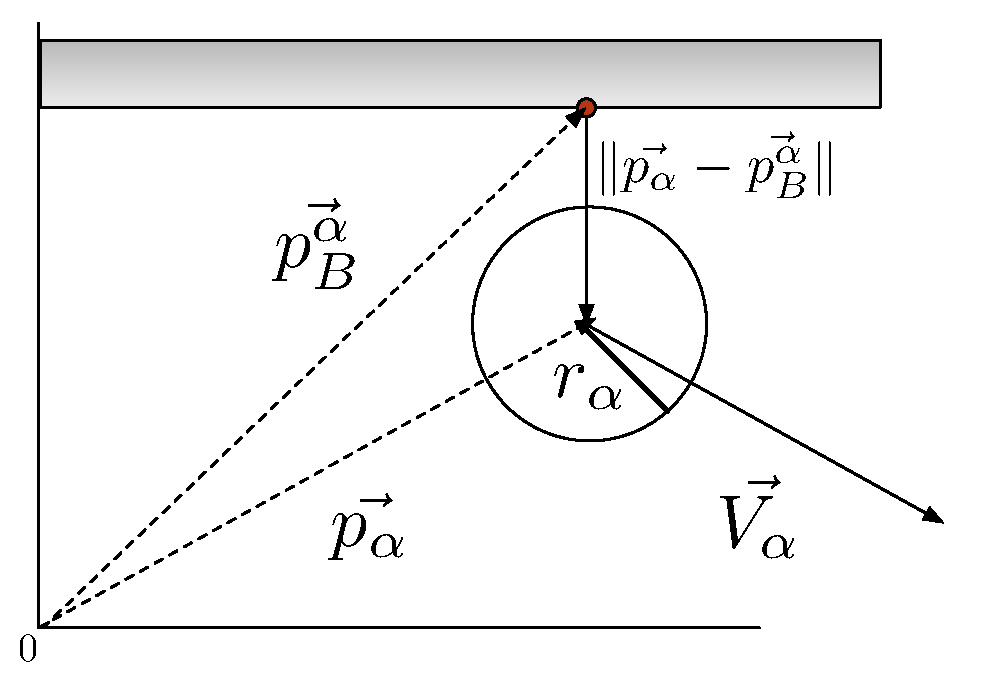
\includegraphics[scale=0.35]{Figures/NotationOfWall.pdf}} 
\caption[Notation of the interaction between an pedestrian and a wall]{The illustration shows the mathematical notation for the interaction with walls used. The circle is pedestrian $\alpha$ with radius $R_{\alpha}$, $\overrightarrow{p_{\alpha}}$ is the position vector for $\alpha$, the grey box on the top is the wall, $\overrightarrow{p_{B}^{\alpha}}$ is the position vector for the closest part of the wall to $\alpha$, $\left( \| \overrightarrow{p_{\alpha}} - \overrightarrow{p_{B}^{\alpha}} \| \right)$ is the smallest distance from $\alpha$ to the wall and $\overrightarrow{V_{\alpha}}$ is the velocity vector for $\alpha$.}
\label{NotationOfWall}
\end{figure}

In order to do the actual calculation we need to know the explicit expression for 
$ \| \overrightarrow{p_{\alpha}} - \overrightarrow{p_{B}^{\alpha}} \|$. First we need to find point on the wall 
that is perpendicular to $\alpha$ as this will be the nearest point to $\alpha$. If we define 
the wall as a vector, $\overrightarrow{W}$ going from a point in space $w_1$ to another point $w_2$, then 
we can find the projection of $\alpha$'s position onto the wall and this projection will be 
$\overrightarrow{p_{B}^{\alpha}}$. This projection is given by:

\begin{equation}\label{wall}
\overrightarrow{p_{B}^{\alpha}}=\frac{\overrightarrow{p_{\alpha}}\cdot \overrightarrow{W}}{\| \overrightarrow{W} \|^2}\overrightarrow{W}
\end{equation}

With this we now have the two points we need to calculate $\|\overrightarrow{p_{\alpha}} - \overrightarrow{p_{B}^{\alpha}}\|$ 
since the position of $\alpha$ is know at all times.

With the explicit expression for $ \| \overrightarrow{p_{\alpha}} - \overrightarrow{p_{B}^{\alpha}} \| $ 
in hand we are able to calculate $\overrightarrow{f_{\alpha B}} \left( \overrightarrow{p_{\alpha}} \right)$ from 
Equation \ref{wallpotential}, as long as the expression for the potential function 
$U_{B}\left( \| \overrightarrow{p_{\alpha}} - \overrightarrow{p_{B}^{\alpha}} \| \right)$ is given. This is 
however not the case in the main article we are working with. In another articles \cite{ABconstant} by 
the same author the repulsive potential from the wall is given by: 

\begin{equation}
U_{B} \left( \| \overrightarrow{p_{\alpha}} - \overrightarrow{p_{B}^{\alpha}} \| \right) =
U^0_{\alpha B} e^{- \| \overrightarrow{p_{\alpha}} - \overrightarrow{p_{B}^{\alpha}} \| / R_{\alpha} }
\end{equation}

where $U^0_{\alpha B}$ is a constant and $R_{\alpha}$ is the radius of a pedestrian $\alpha$.
In that case, the repulsive force on pedestrian $ \alpha $ from the wall is:

\begin{equation}
    \overrightarrow{f_{\alpha B}} \left( \overrightarrow{p_{\alpha}} \right) =
    - \nabla_{\overrightarrow{p_{\alpha}}} U_{B}
    \left( \| \overrightarrow{p_{\alpha}} - \overrightarrow{p_{B}^{\alpha}} \| \right)\\
=-\left( \frac{\partial}{\partial x_{\alpha}}U_{B}( \| \overrightarrow{p_{\alpha}} - \overrightarrow{p_{B}^{\alpha}} \|), \frac{\partial}{\partial y_{\alpha}}U_{B}( \| \overrightarrow{p_{\alpha}} - \overrightarrow{p_{B}^{\alpha}} \|)\right)
\end{equation}

Calculating the derivatives we assume that we now the direction of the force, so the differentiation will be one dimensional

\begin{equation}
\begin{split}
f_{\alpha B} \left( \overrightarrow{p_{\alpha}} \right) 
 = -\frac{\partial}{\partial \| \overrightarrow{p_{\alpha}} - \overrightarrow{p_{B}^{\alpha}} \|}U^0_{\alpha B} e^{- \| \overrightarrow{p_{\alpha}} - \overrightarrow{p_{B}^{\alpha}} \| / R_{\alpha} }
\end{split}
\end{equation}

The differentiation then gives: 

\begin{equation}
    f_{\alpha B} \left( \overrightarrow{p_{\alpha}} \right) 
=\frac{1}{R_{\alpha}} U^0_{\alpha B} e^{- \| \overrightarrow{p_{\alpha}} - \overrightarrow{p_{B}^{\alpha}} \| / R_{\alpha} }
\end{equation}

To get the direction of the force, we multiply it with the unit vector of the vector from the wall to $\alpha$ since the force will have the same direction 
\begin{equation}\label{eqn:wall-repulsion}
\overrightarrow{f_{\alpha B}}=\frac{1}{R_{\alpha}} U^0_{\alpha B} e^{- \| \overrightarrow{p_{\alpha}} - \overrightarrow{p_{B}^{\alpha}} \| / R_{\alpha} }\frac{\left(p_{\alpha x}-p_{Bx}^{\alpha },p_{\alpha y}-p_{By}^{\alpha }\right)}{ \| \overrightarrow{p_{\alpha}} - \overrightarrow{p_{B}^{\alpha}} \| }
\end{equation}

The exponential function will always lay between 0 and  1:

\begin{equation}
0 < e^{ -\| \overrightarrow{p_{\alpha}} - \overrightarrow{p_{B}^{\alpha}} \| /R_\alpha} < 1
\end{equation}

Which leads to:

\begin{equation}
0< U_{B} \left( \| \overrightarrow{p_{\alpha}} - \overrightarrow{p_{B}^{\alpha}} \| \right) < U^0_{\alpha B}
\end{equation}

We can see that this force act in the following way: $\overrightarrow{f_{\alpha B}}$ tends to 0 as the distance 
$\| \overrightarrow{p_{\alpha}} - \overrightarrow{p_{B}^{\alpha}} \|$ gets large, meaning that a pedestrian in a reasonably 
distance from the wall will feel a diminishing force. $\overrightarrow{f_{\alpha B}}$ tends to $U^0_{\alpha B}$ 
as the distance $ \| \overrightarrow{p_{\alpha}} - \overrightarrow{p_{B}^{\alpha}} \|$ tends to $0$ the pedestrian will be 
pushed, with some force depending on $U^0_{\alpha B}$, away from the wall. The negative of the force 
means that when the potential between wall and pedestrian rises so will the force, but in the opposite 
direction meaning that the pedestrian will be pushed away. This can be understood as if the pedestrian 
is trying to avoid the wall as it is expected from real life situations. \cite{social-force}. %real references, please.

\begin{center}
\begin{tabular}{lll}
\hline
$\overrightarrow{p_{\alpha}^{\text{B}}}$& Vector pointing from origo to the point on the wall nearest to pedestrian alpha &\\
\hline
$\overrightarrow{W}$& Vector representing the wall &\\
\hline
$U_{B}$ & Repulsive potential from the wall\\
\hline
$U^{0}_{\alpha B}$ & Constant representing pedestrian alpha's tendency to avoid walls\\
\hline
$R_{\alpha}$& Repulsive potential from the wall\\
\hline
\end{tabular}
\end{center}

\subsection{Summary of the model}
\begin{figure}[hb] %with some more comments i think that this figure could serve as a summation of the entire section
    \centering
    {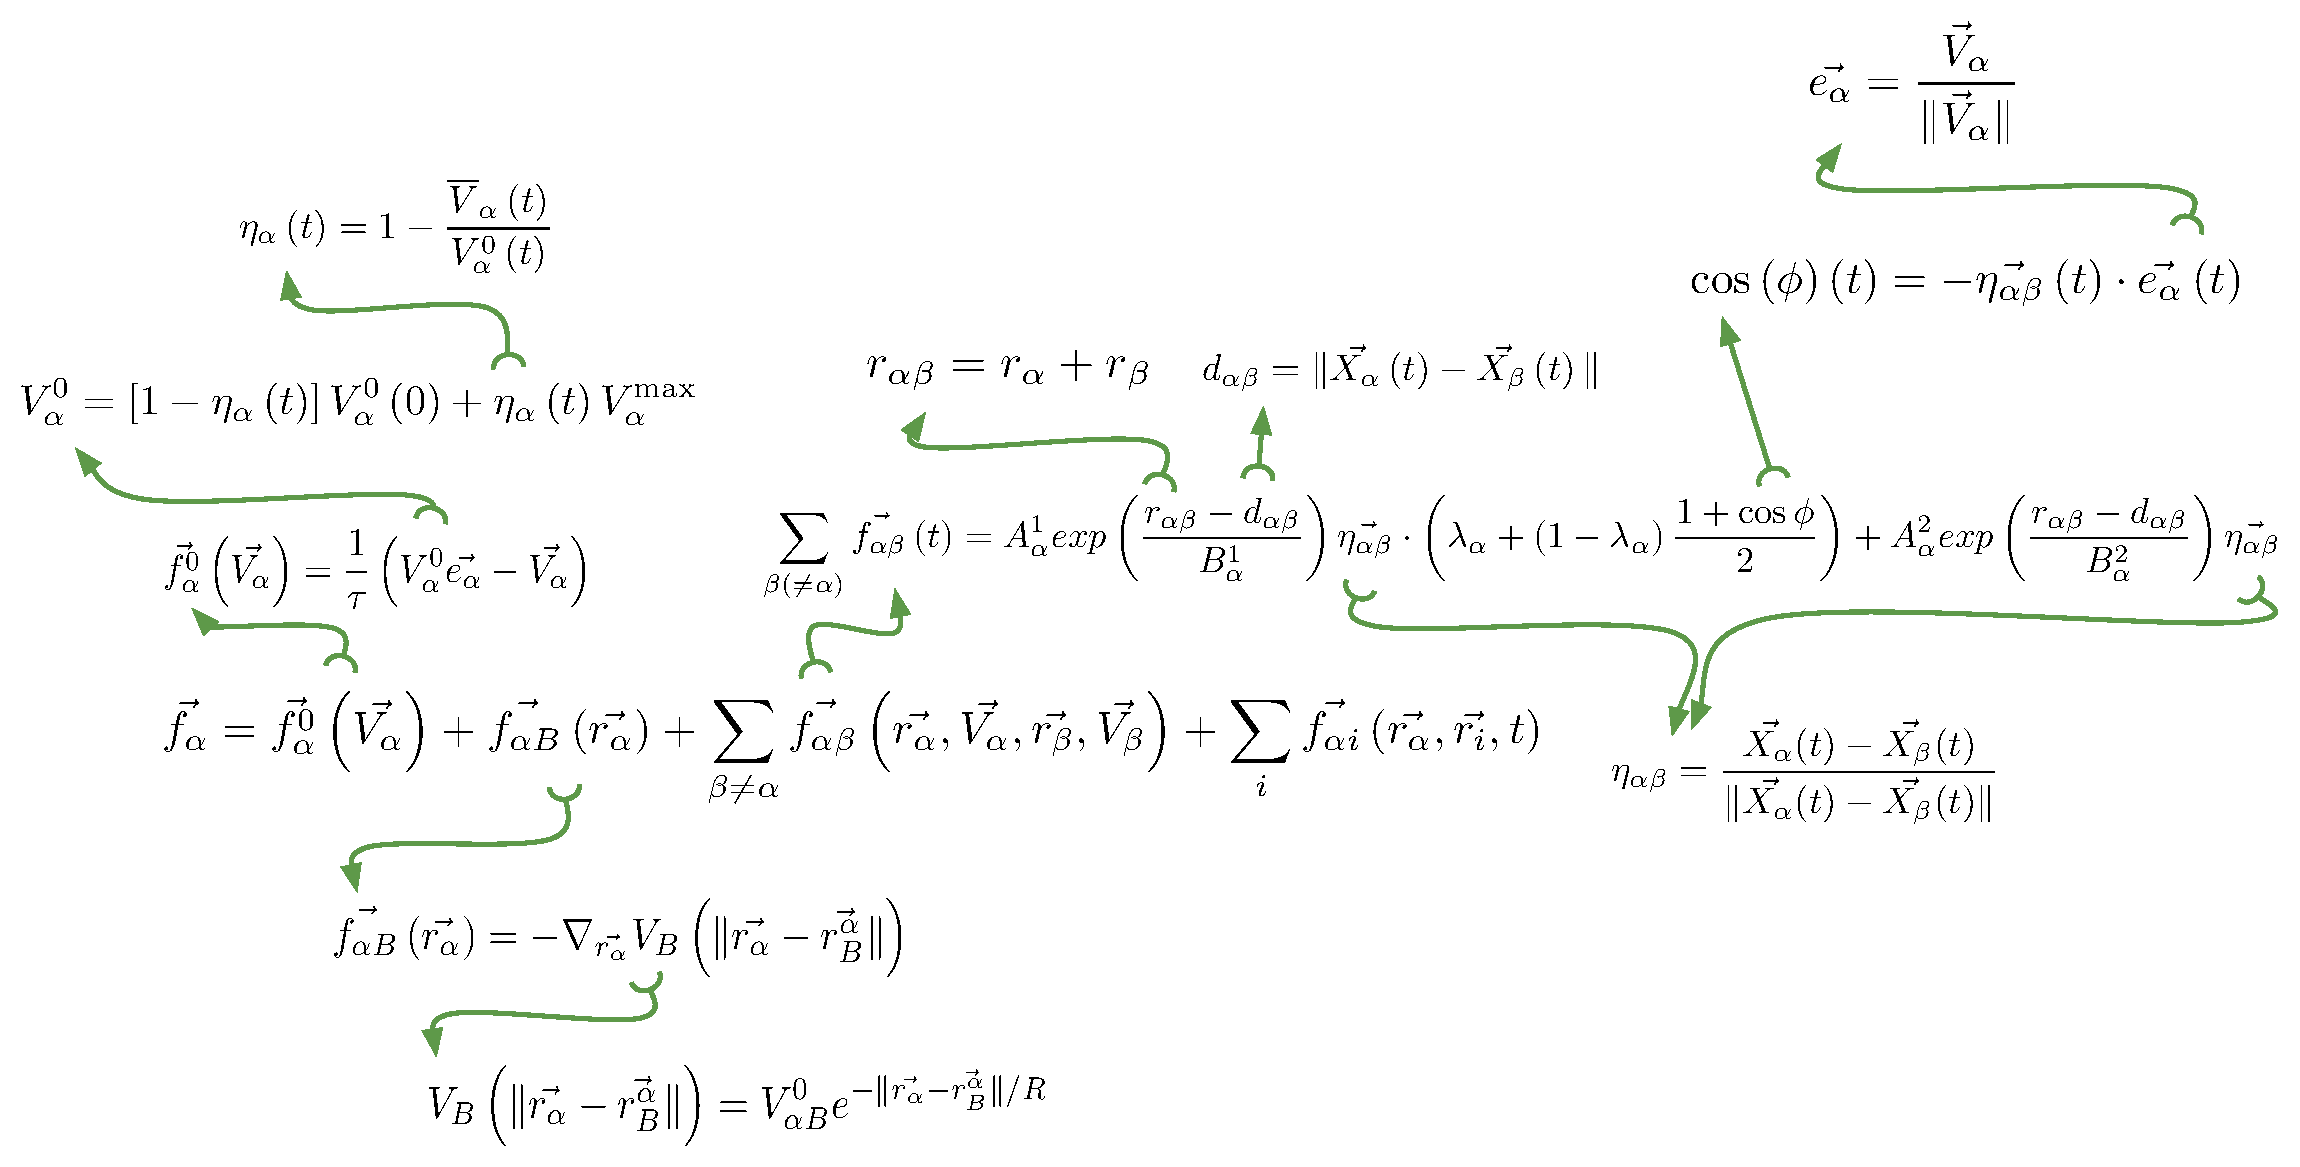
\includegraphics[scale=0.35]{Figures/overview.pdf}} 
    \caption[Overview of the model]{Illustration of an overview of how the model is put together. The different equations and their notation is written to give the 
	     reader an overview of how the model looks like.}
    \label{overview}
\end{figure}

\begin{center}
\begin{tabular}{lll}
\hline
$\overrightarrow{f_{\alpha}^{0}}$ & the desired force &\\
\hline
$\overrightarrow{f_{\alpha B}}$ & the repulsive force from walls &\\
\hline
$\overrightarrow{f_{\alpha \beta}}$ & the repulsion from other pedestrians\\
\hline
$\overrightarrow{f_{\alpha i}}$& the attractive force\\
\hline
$\overrightarrow{V_{\alpha}}$ & The actual velocity of pedestrian alpha &\\
\hline
$V_{\alpha}^{0}(t)$ & The desired speed of pedestrian alpha &\\
\hline
$V_{\alpha}^{0}(0)$ & The initial desired speed of pedestrian alpha &\\
\hline
$\overline{V_{\alpha}(t)}$ & The average speed of pedestrian alpha &\\
\hline
$\overrightarrow{p_{\alpha}}$ & The position vector of pedestrian alpha\\
\hline
$e_{\alpha}$& The desired direction of pedestrian alpha\\
\hline
$\tau$& The relaxation time &\\
\hline
$\overrightarrow{p_{\alpha}^{\text{B}}}$& Vector pointing from origo to the point on the wall nearest to pedestrian alpha &\\
\hline
$\overrightarrow{W}$& Vector representing the wall &\\
\hline
$U_{B}$ & Repulsive potential from the wall\\
\hline
$U^{0}_{\alpha B}$ & Constant representing pedestrian alpha's tendency to avoid walls\\
\hline
$R_{\alpha}$& Repulsive potential from the wall\\
\hline
$d_{\alpha \beta}$& The distance from pedestrian $\alpha$ to $\beta$ &\\
\hline
$R_{\alpha\beta}$& The sum of the radii of pedestrian $\alpha$ and $\beta$ \\
\hline
$\lambda_{\alpha}$& Anisotropy parameter &\\
\hline
$\eta_{\alpha \beta}$& Normal vector pointing from $\beta$ to $\alpha$ \\
\hline
$A_{\alpha}$& Parameter controlling the interaction streanght \\
\hline
$B_{\alpha}$& Parameter controlling the range of the repulsive interaction  \\
\hline
$d_{\alpha \beta}$& The distance from pedestrian $\alpha$ to $\beta$ &\\
\hline
$R_{\alpha\beta}$& The sum of the radii of pedestrian $\alpha$ and $\beta$ \\
\hline
$\lambda_{\alpha}$& Anisotropy parameter &\\
\hline
$\eta_{\alpha \beta}$& Normal vector pointing from $\beta$ to $\alpha$ \\
\hline
$A_{\alpha}$& Parameter controlling the interaction streanght \\
\hline
$B_{\alpha}$& Parameter controlling the range of the repulsive interaction  \\
\hline
\end{tabular}
\end{center}

We have now seen the explicit mathematical expression for the social forces 
as well as explained how this affects the behavior of the pedestrians. To get an 
overview of how the model is put together look a figure \ref{overview} with 
the aid of table. In section \ref{sec:assessment} 
we discuss some of the models features in more detail as well as some features 
that the model does not have. For the implementation of the model see section \ref{sec:simulation}.
